%\documentclass[14pt]{beamer}
\documentclass[aspectratio=169]{beamer}
\usetheme[titleformat=regular%
,numbering=fraction% use slide numbers
]{metropolis}
\usepackage{appendixnumberbeamer} % separate appendix
\usepackage[citestyle=authortitle-ibid,sorting=none]{biblatex}
\setbeamerfont{footnote}{size=\tiny}
\addbibresource{mae.bib}

% multimedia in beamer presentations
\usepackage{multimedia}

% adding some better facilities to latex such as proper booleans
\usepackage{etoolbox}

% Unicode math symbols for XeLaTeX
\usepackage{mathrsfs}

% standard math packages
\usepackage{amssymb}
\usepackage{amsthm}
\usepackage{amsmath}
\usepackage{amstext}
\usepackage{mathabx}
\usepackage{stmaryrd}
% math tools for amsmath
\usepackage{mathtools}

\usepackage{proof}

\usepackage{listings}
\usepackage{xcolor}

% subfigures, subfloats
\usepackage{subcaption}

% for multiinclude
\usepackage{xmpmulti}

% tikz & friends

\usepackage{galois}
\usepackage{tikz}
\usetikzlibrary{fit,calc,shapes,arrows.meta,patterns,backgrounds}
\usetikzlibrary{decorations.pathmorphing}
\usetikzlibrary{cd}
\usepackage[beamer]{hf-tikz}

\newcommand{\tikzmark}[1]{%
  \tikz[overlay,remember picture,baseline] \node [anchor=base] (#1) {};}

\newenvironment{tightcenter}{%
  \setlength\topsep{0pt}
  \setlength\parskip{0pt}
  \begin{center}
}{%
  \end{center}
}

% new colors
\definecolor{lightblue}{RGB}{217,220,253}
\definecolor{lightred}{RGB}{251,216,218}

\DeclareMathOperator{\pw}{\mathcal{P}} % powerset
\newcommand{\fset}[1]{\mathsf{#1}}
\newcommand{\nats}{\mathbb{N}}
\newcommand{\zahlen}{\mathbb{Z}}
\newcommand{\bools}{\mathbb{B}}
\newcommand{\Set}[1]{\left\{#1\right\}}
\newcommand{\true}{\kw{true}}
\newcommand{\false}{\kw{false}}
\newcommand{\sidenote}[1]{\hfill\quad \textsf{#1}}

\newcommand{\disunion}{+}

% named set
\newcommand{\ns}[1]{\mathit{#1}}
% function
\newcommand{\fn}[1]{\mathrm{#1}}
% "vector of"
\newcommand{\vo}[1]{\overrightarrow{#1}}
% "set of"
\newcommand{\setOf}[1]{\overline{#1}}
% syntactic tag
\newcommand{\sTag}[2]{\textsf{\textbf{#1}}\,#2}
% keyword
\newcommand{\kw}[1]{\texttt{#1}}
% usual suspects
\newcommand{\State}{\ns{State}}
\newcommand{\Value}{\ns{Value}}
\newcommand{\Stmt}{\ns{Stmt}}
\newcommand{\Env}{\ns{Env}}
\newcommand{\Store}{\ns{Store}}
\newcommand{\Kont}{\ns{Kont}}
% syntactic domains
\newcommand{\Exp}{\ns{Exp}}
\newcommand{\Var}{\ns{Var}}
\newcommand{\Addr}{\ns{Addr}}
% put a value to a pointer
\newcommand{\update}{\leftarrow}

% ebnf
\newcommand{\eDEF}{\,::=\;}
\newcommand{\eOR}{\;\vert\;}

\newcommand{\widen}{\nabla}

% \newcommand{\|}{\,\vert\,}

\newcommand{\todo}[1]{\iftoggle{TODO}{\textcolor{red}{TODO: #1}}{}}
% ceiling and floor symbols
\DeclarePairedDelimiter\ceil{\lceil}{\rceil}
\DeclarePairedDelimiter\floor{\lfloor}{\rfloor}

% big O notation
\DeclareMathOperator{\bigO}{O}

% fixed points
\DeclareMathOperator{\lfp}{lfp}

% print both years for bibliography
\renewbibmacro*{cite:labelyear+extrayear}{%
\iffieldundef{labelyear}
{}
{\printtext[bibhyperref]{%
\iffieldundef{origyear}{}{\printfield{origyear}\addslash}%   <--- added
\printfield{labelyear}%
\printfield{extrayear}}}}

\renewbibmacro*{date+extrayear}{%
\iffieldundef{year}
{}
{\printtext[parens]{%
\iffieldundef{origyear}{}{\printfield{origyear}\addslash}%  <--- added
\printdateextra}}}

% overlay an image
\def\Put(#1,#2)#3{\leavevmode\makebox(0,0){\put(#1,#2){#3}}}

% text over symbols nicely, requires amsmath for overset
\newcommand\textoverop[2]{\mathrel{\overset{\makebox[0pt]{\mbox{\normalfont\tiny\sffamily #1}}}{#2}}}

% special arrows
\newcommand\monarrow{\textoverop{mon}{\rightarrow}}

% theorems
\newtheorem{thm}{Theorem}
\newtheorem{eg}{Example}

\newcommand{\abscolor}[1]{\textcolor{mLightBrown}{#1}}
\newcommand{\concolor}[1]{\textcolor{mLightGreen}{#1}}
\newcommand{\abst}[1]{#1^{\#}}

\newcommand{\step}{\rightsquigarrow}

% listings setup
\lstset{basicstyle=\tiny\ttfamily,columns=fixed}

%%% Local Variables:
%%% mode: latex
%%% TeX-master: "main"
%%% TeX-engine: xetex
%%% End:


\title[Major Area Exam]{Abstract Interpretation of Low-level Programs}
\subtitle{Major Area Exam}
\date{January 23, 2018}
\author{Mehmet Emre}
\institute[UCSB]{
  \normalsize
  {\large \bfseries Committee:}\\
  Ben Hardekopf (\,$\vcenter{\hbox{
\includegraphics[height=1em]{chair/file.eps}}}$) \quad
  Tevfik Bultan \quad
  Chandra Krintz
}
\titlegraphic{\hfill
\includegraphics[width=2.25cm]{ucsbseal_cmyk.pdf}}

\begin{document}
\maketitle

\begin{frame}{Outline}
  \small
  \vspace{0.5em}
  \tableofcontents
\end{frame}

\section{Introduction}
\begin{frame}{What is low-level software? Why should we analyze it?}
Low-level software:
\begin{itemize}
\item Interacts with intricate APIs (drivers, kernel modules, databases)
\item Require preserving subtle invariants (above, control software)
\item Have heavy reliability requirements
\begin{itemize}
\item with unpleasant consequences % : BSoD, data loss, Arianne~5, Heartbleed, Patriot missile
\end{itemize}
\end{itemize}

\end{frame}

\only<beamer>{ % all template changes are local to this group.
  \setbeamertemplate{navigation symbols}{}
  \begin{frame}[plain]
    \begin{tikzpicture}[remember picture,overlay]
      \node[at=(current page.center)] {
        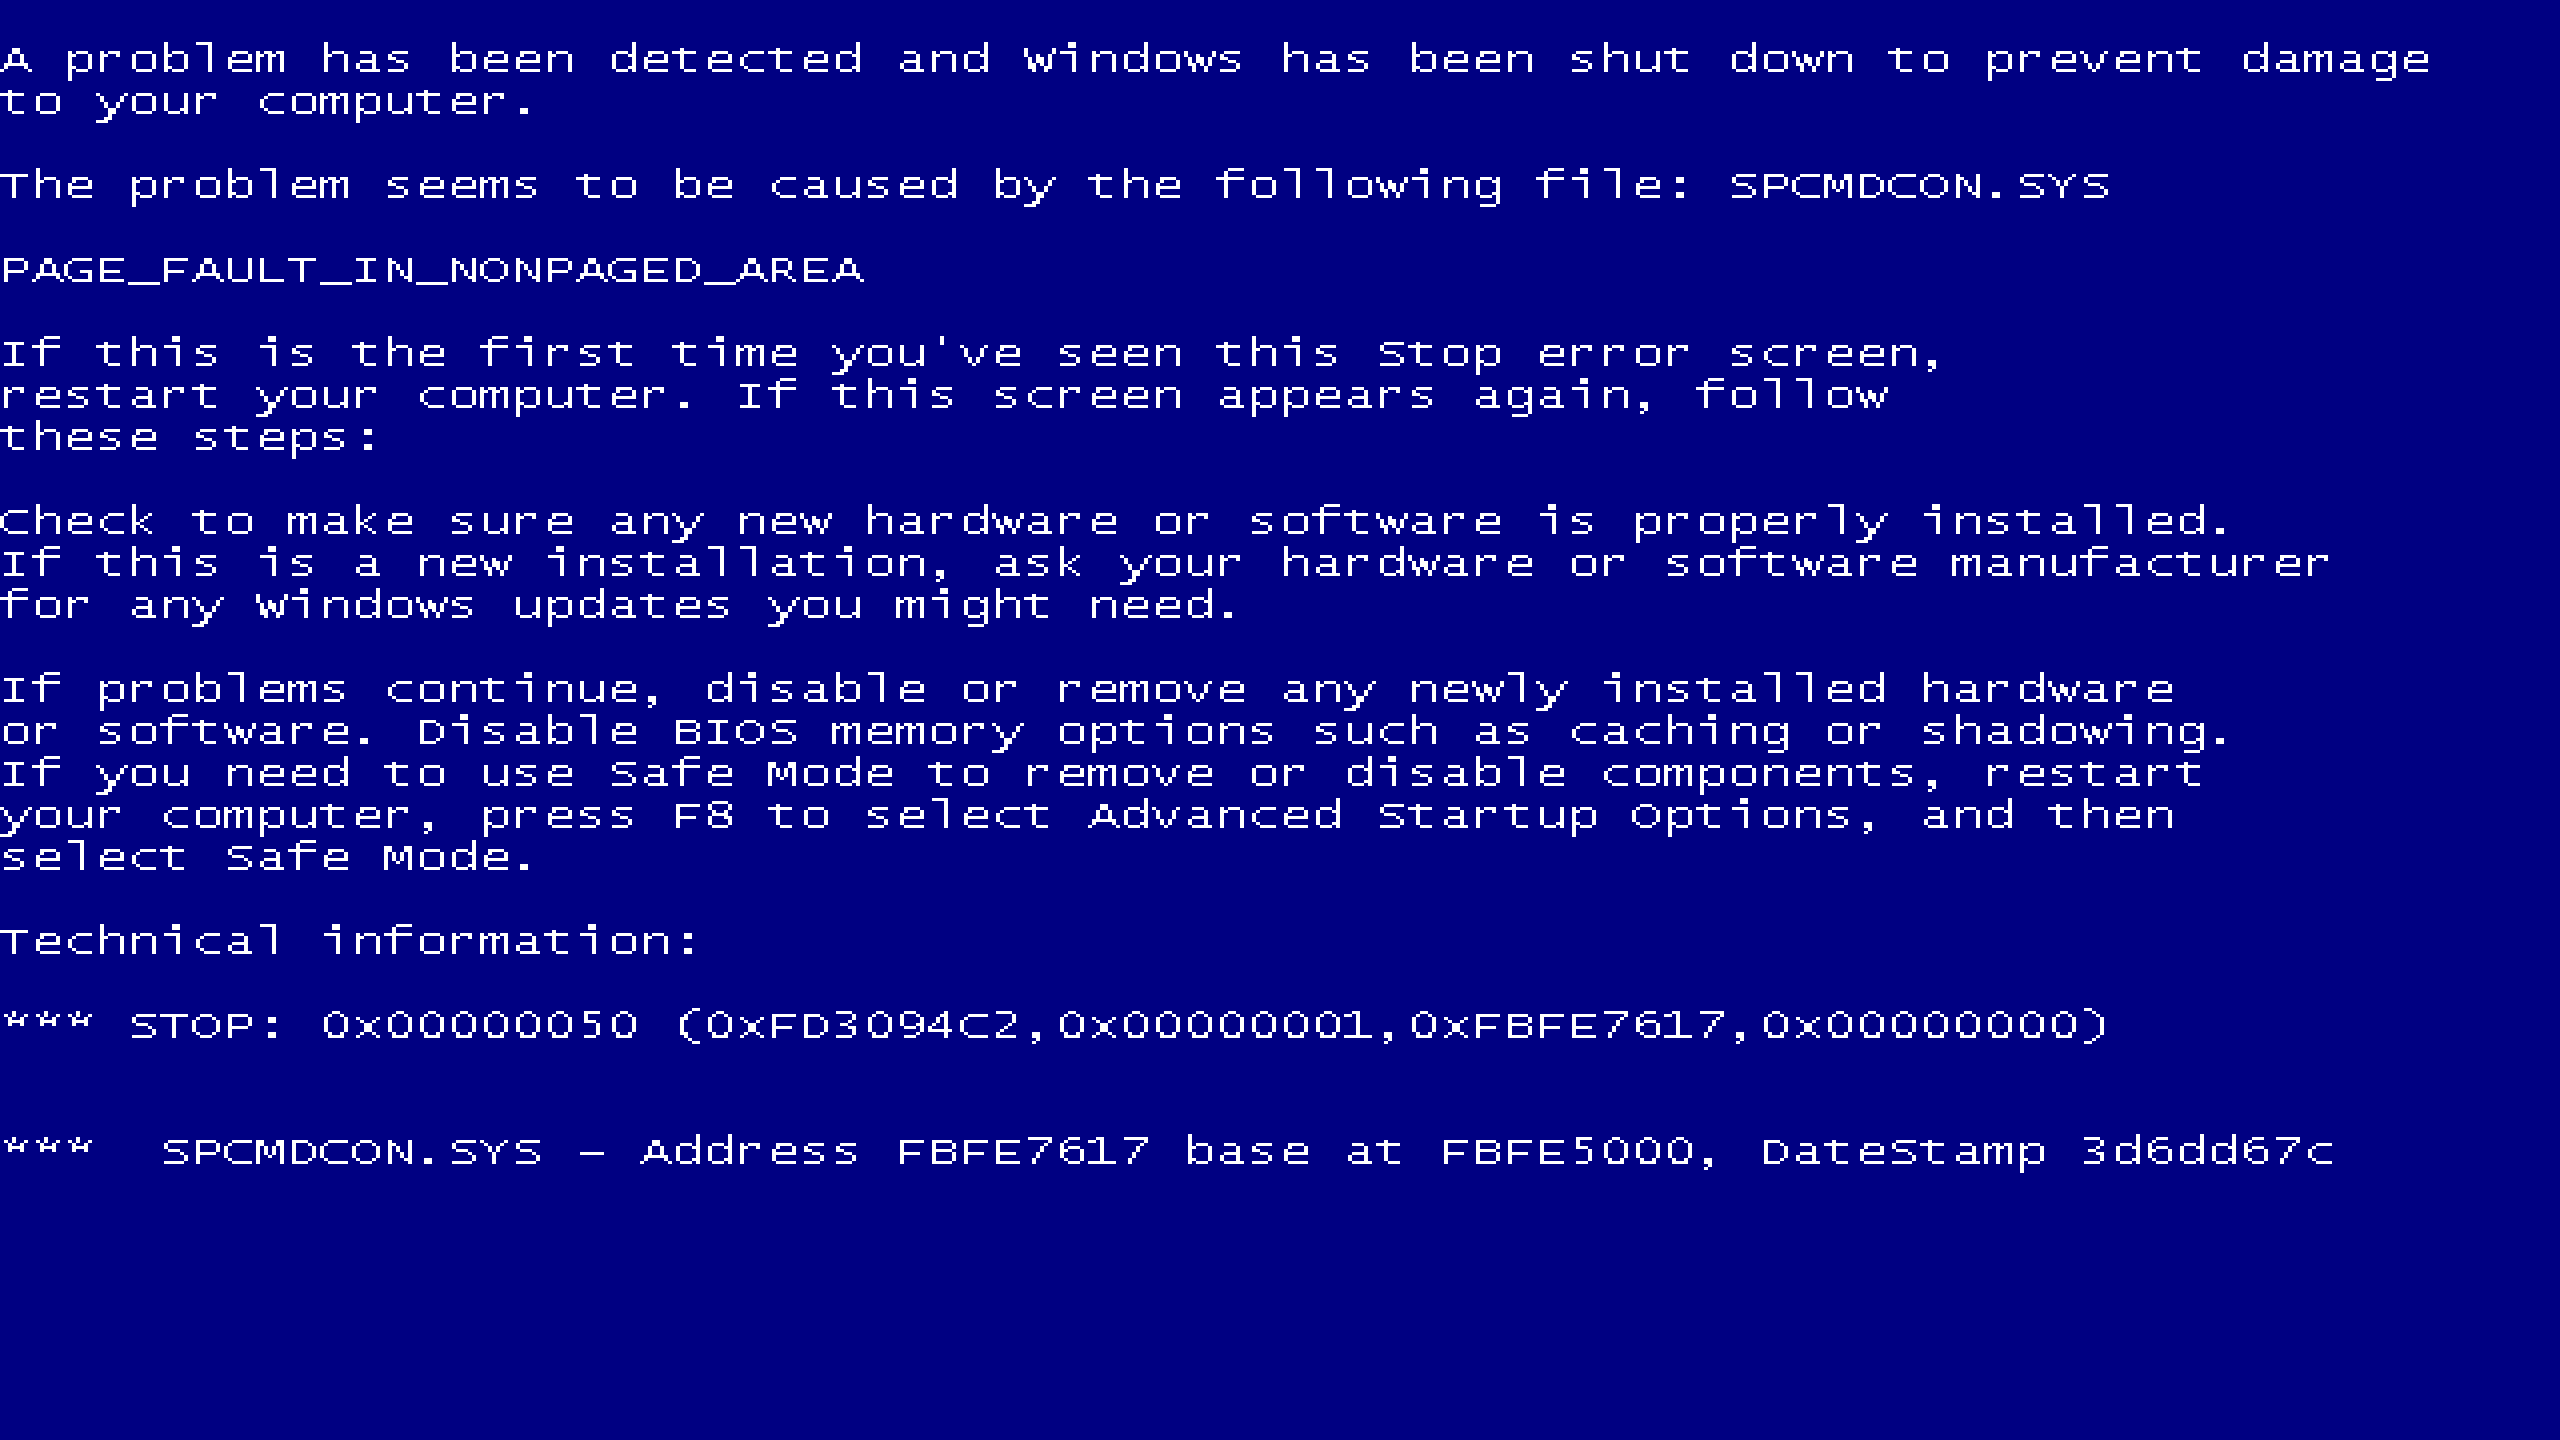
\includegraphics[width=\paperwidth]{material/bsod_resized.png}
      };
    \end{tikzpicture}
    %\sound[autostart,inlinesound]{foo}{beep.wav}
    \pause
    \Put(10,10){
\includegraphics[width=0.4\textwidth]{material/heartbleed.pdf}}\pause
    \Put(180,200){
\includegraphics[width=0.4\textwidth]{material/formal-verification-as-a-sinking-airplane.png}}\pause
    \Put(210,-100){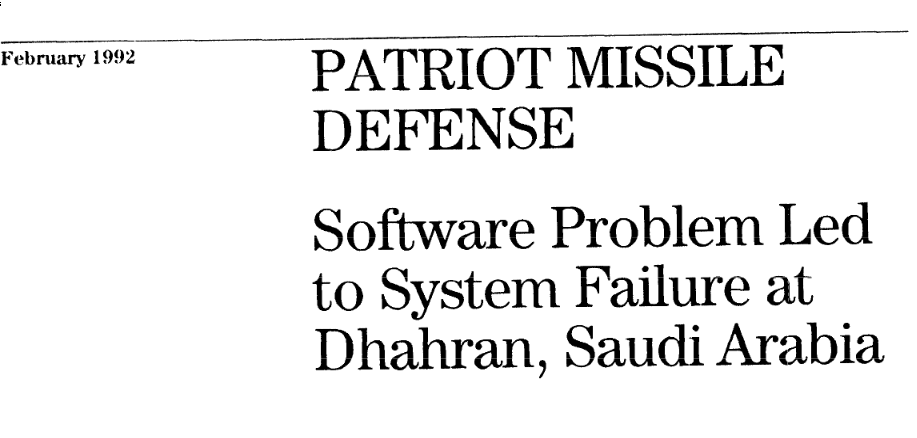
\includegraphics[width=0.5\textwidth]{material/us-govt-patriot-missile.png}}
  \end{frame}
}

\only<handout>{
  \addtocounter{framenumber}{1}
}


\begin{frame}{Why abstract interpretation?}
There are other alternatives:
\begin{itemize}[<+->]
\item ad-hoc, iterative DFA (not amenable to systematic correctness)
\item model checking (there is a neat connection with model checking)
\item type systems (limits choice of language, context-insensitive)
\end{itemize}
\end{frame}

\section{A first attempt}
\begin{frame}{SIMPL\footnote{simple introductory made-up programming language} Syntax}
  \vspace{-2em}
  \small
  \begin{gather*}
    x,f \in \Var,\, b \in \bools,\, n \in \zahlen,\, \oplus \in \ns{BinOp},\,\Value = \bools \disunion \zahlen
  \end{gather*}\vspace{-2em}
  \begin{align*}
    fd \in \ns{FunDef} \eDEF & \alert<5>{\kw{def}\; f(\vo{x}) = s;\,\kw{return}\; e} \\
    e \in \Exp \eDEF & x \eOR n \eOR b \eOR e_1 \oplus e_2 \eOR *x \eOR \alert<1>{\kw{choose}\;e_1\,e_2} \\
    s \in \Stmt \eDEF & s;\,s \eOR \alert<2>{\kw{abort}} \\
    \eOR & \alert<4>{\kw{if}\, e\; s_1 \; \kw{else} \; s_2} \\
    \eOR & \alert<4>{\kw{while}\; e\; s} \\
    \eOR & \kw{let}\; x := e \;\kw{in}\;s \\
    \eOR & \alert<3>{\kw{letref}\; x := \kw{new}\;e \;\kw{in}\;s} \\
    \eOR & \alert<3>{e_1 \update e_2} \eOR x := e \\
    \eOR & \alert<5>{x := f(\vo{e})}
  \end{align*}
\end{frame}
\begin{frame}{SIMPL semantic domains}
  \begingroup\footnotesize We will use abstract machine semantics and represent the semantics of a program as a transition relation.\endgroup
\begin{align*}
    \varsigma \in \State & = \Stmt^? \times \Env \times \Store \times \alert<4>{\Kont} \\
    \rho \in \Env & = \alert<2>{\Value}^{\alert<3>{\Var}} \only<1>{\alert{= \Set{\rho : \Var \to \Value}}} \\
    \sigma \in \Store & = \alert<2>{\Value}^{\alert<3>{\Addr}} \\
    \kappa \in \alert<4>{\Kont} & = \sTag{stmtK}{\Stmt \times \alert<4>{\Kont}} \\
                         & \disunion \sTag{whileK}{\Exp \times \Stmt \times \alert<4>{\Kont}} \\
                         & \disunion \sTag{retK}{\Var \times \Exp \times \Env \times \alert<4>{\Kont}}
\end{align*}
\end{frame}

\begin{frame}{Some transition rules}
  \small
  \begin{itemize}
  \item $\varsigma \step \varsigma'$ is the transition relation\footnote{Because of nondeterminism. One can also view it as a transition \emph{function} from a state to a set of states.}
  \item \(\eta_\varsigma : \Exp \to \Value \) is the per-state expression evaluation function
\item Current state: \(\varsigma = (so, \rho, \sigma, \vec{\kappa})$ and $\kappa :: \vec{\kappa_r} = \vec{\kappa} \)
\item Next state: \( \varsigma' = (so', \rho', \sigma', \vec{\kappa}') \) \pause
  \end{itemize}
  \footnotesize
  \[
  \begin{array}{llllll}
    so & \text{side condition} & so' & \rho' & \sigma' & \vec{\kappa}' \\ \hline
    e_1 \update e_2 & & - & \rho & \sigma[\eta_\varsigma(e_1) \mapsto \eta_\varsigma(e_2)] & \vec{\kappa} \\
    \kw{while}\; e\; s & \eta_\varsigma(e) = \true & - & \rho & \sigma & \sTag{stmtK}{s} :: \sTag{whileK}{(e, s)} :: \vec{\kappa} \\
    \kw{while}\; e\; s & \eta_\varsigma(e) = \false & - & \rho & \sigma & \vec{\kappa} \\
    - & \kappa = \sTag{stmtK}{s} & s & \rho & \sigma & \vec{\kappa_r}
  \end{array}
  \]
\end{frame}

\begin{frame}{Collecting semantics}
  Abstract machine semantics gives us a state transition system $(\State, I, \step)$ where \pause $\State$ is the set of states, \pause $I \subset \State$ is the set of initial states, \pause $\step \subset \State \times \State$ is the transition relation. \pause Let
  \[ F : \pw(\State) \monarrow \pw(\State),\, F(X) = \Set{y \vert (x, y) \in \step \wedge x \in X}. \]\pause
  $\lfp_I F = I \cup F(I) \cup F(F(I)) \cup \ldots $ is the set of reachable states.\pause

  \alert{$\lfp_I F$ is potentially infinite and requires infinitely many steps to compute!}
\end{frame}

\section{Lattices and order}

\begingroup
\small
\begin{frame}{Lattices and Order Theory}
  \vspace*{-1em}
  \begin{columns}[T]
  \begin{column}{0.6\textwidth}
  \begin{itemize}
  \item A lattice $(L, \sqcup, \sqcap, \sqsubseteq)$ is a partially ordered set (poset) with:\vspace{-0.8em}
    \begin{itemize}
    \item a least upper bound (join) operation $\sqcup: L \times L \to L$
    \item a greatest lower bound (meet) operation $\sqcap: L \times L \to L$
    \item $\sqcup, \sqcap$ determine the partial order $\sqsubseteq$
    \end{itemize}\vspace{-1em}
  \item<9-> A bounded lattice has a least element $\bot$, (bottom)
    and greatest element $\top$ (top)\vspace{-1em}
  \item<10-> Any powerset $\mathcal{P}(S)$ of a set $S$ is a bounded lattice where:
     $\top = S$,
     $\bot = \emptyset$,
     $\sqcup = \cup$,
     $\sqcap = \cap$,
     $\sqsubseteq = \subseteq$
  \end{itemize}\
  \end{column}
  \begin{column}{0.4\textwidth}
    \begin{figure}[h]
    \centering
    \begin{tikzpicture}[x=2cm, y=1.5cm]
      \node(top)at (1,3){$\textcolor<9>{magenta}{\{+,-,0\} = \top}$} ;
      \node(pm)at (1,2){$\{+,-\}$} ;
      \node(mz)at (2,2){$\{-,0\}$} ;
      \node(pz)at (0,2){$\textcolor<4>{magenta}{\{+,0\}}$} ;
      \node(p)at (0,1){$\{+\}$} ;
      \node(m)at (2,1){$\{-\}$} ;
      \node(z)at (1,1){$\textcolor<8>{magenta}{\{0\}}$} ;
      \node(bot)at (1,0){$\textcolor<9>{magenta}{\emptyset = \bot}$} ;
      \draw(top)--(pm);
      \draw(top)--(mz);
      \draw(top)--(pz);
      \draw(pm)--(p);
      \draw(pm)--(m);
      \draw(mz)--(m);
      \draw[onslide={<7-8> draw=magenta, line width=1.2pt}](mz)--(z);
      \draw[onslide={<2-4> draw=magenta, line width=1.2pt}](pz)--(p);
      \draw[onslide={<3-4,6-8> draw=magenta, line width=1.2pt}](pz)--(z);
      \draw(p)--(bot);
      \draw(m)--(bot);
      \draw(z)--(bot);
    \end{tikzpicture}
    \caption{\footnotesize Hasse diagram of a sign lattice, built from the powerset of the set $\{+,-,0\}$}
  \end{figure}
  % \only<4>{\begin{figure}[t]
  %   \centering
  %   \begin{tikzpicture}[x=1.25cm, y=1.25cm]
  %     \node(top)at (0,1){$\top$} ;
  %     \node(e)at (-1,0){$e$} ;
  %     \node(o)at (1,0){$o$} ;
  %     \node(bot)at (0,-1){$\bot$} ;
  %     \draw(top)--(o)--(bot);
  %     \draw(top)--(e)--(bot);
  %   \end{tikzpicture}
  %   \caption{Hasse diagram of an even/odd lattice}
  % \end{figure}}
  \end{column}
  \end{columns}
\end{frame}
\endgroup % footnotesize

\begingroup
\footnotesize
\begin{frame}{Relating lattices}
  \vspace*{-1.2em}
  \begin{columns}[t]
    \begin{column}{0.7\textwidth}
    \begin{itemize}
    \item There is a relationship between $\mathit{Parity}$ and
      $\mathcal{P}(\mathbb{Z})$:\vspace{-0.8em}
      \begin{align*}
        \uncover<2->{\gamma : \mathit{Parity} & \monarrow \mathcal{P}(\mathbb{Z}) \\
        \alpha : \mathcal{P}(\mathbb{Z}) & \monarrow \mathit{Parity}}
      \end{align*}\vspace{-3em}
      \begin{align*}
        \uncover<3->{\gamma(\top) & = \mathbb{Z}, \gamma(\bot) = \emptyset \\
        \gamma(o) & = \{z \in \mathbb{Z} \mid z \text{ odd} \} \\
        \gamma(e) & = \{z \in \mathbb{Z} \mid z \text{ even} \}} \\
        \uncover<4->{\alpha(S) & = \bigsqcup\limits_{z \in S}
        \begin{cases}
          o & z \text{ odd}\\
          e & z \text{ even}
        \end{cases}}
      \end{align*}\vspace{-2em}
    \item<5-> $\alpha$ and $\gamma$ are kind of like inverses, though
      there is some information loss\vspace{-0.6em}
    \item<6-> $\alpha$ happens to be the \emph{best possible} function to pair
      with $\gamma$ in a certain sense\vspace{-0.6em}
    \item<7-> This relationship is known as a \alert{\emph{Galois Connection}}
    \end{itemize}
  \end{column}
  \begin{column}{0.3\textwidth}
    \begin{figure}
      \centering
      \footnotesize
      \begin{tikzpicture}[x=1.25cm, y=1.25cm]
        \node(top)at (0,1){$\top$} ;
        \node(e)at (-1,0){$e$} ;
        \node(o)at (1,0){$o$} ;
        \node(bot)at (0,-1){$\bot$} ;
        \draw(top)--(o)--(bot);
        \draw(top)--(e)--(bot);
      \end{tikzpicture}\\[0.5em]

      \onslide<4->{$\alert<4>{\alpha(5) + \alpha(-7) = e + o = o}$}
      \caption{\footnotesize Hasse diagram of an even/odd lattice ($\mathit{Parity}$), and
        an example of abstracting an operator}
    \end{figure}
  \end{column}
  \end{columns}
\end{frame}
\endgroup

\begingroup
\small
\begin{frame}{Galois Connections}
  \[ \textcolor<2->{gray}{\forall c \in \mathit{Concrete}, a \in \mathit{Abstract}.\, c \subseteq \gamma(a) \iff \alpha(c) \sqsubseteq a} \]
  \pause
  or, equivalently,
  $$ \tikzmark{ma}\textcolor<1,7->{gray}{\alpha, \gamma \text{ monotone}}\tikzmark{mb} \qquad \tikzmark{a}\textcolor<1,4-6,10->{gray}{c \subseteq \gamma(\alpha(c))}\tikzmark{b} \qquad \tikzmark{ra}\textcolor<1,4-9>{gray}{\alpha(\gamma(a)) \sqsubseteq a\tikzmark{rb}} $$
  \pause
  \vspace*{-1em}
  \begin{tightcenter}
   \begin{tikzpicture}
     \draw[fill=lightblue] (0,0.25) ellipse (1.75cm and 1.75cm);
     \node at (0,2.33) {$\mathcal{P}(\mathbb{Z})$};
     \node at (5.5,1.5) {$\mathit{Parity}$};

     \node(top)at (5.5,1){$\top$} ;
     \node(e)at (4.5,0){$e$} ;
     \node(o)at (6.5,0){$o$} ;
     \node(bot)at (5.5,-1){$\bot$} ;
     \draw(top)--(o)--(bot);
     \draw(top)--(e)--(bot);

     \node (z) at (0,1.75) {$\mathbb{Z}$};
     \node (evens) at (-.75,1) {$evens$};
     \node (odds) at (.75,1) {$odds$};
     \node (two) at (0,-0.5) {$\{ 2 \}$};
     \node (empty) at (0,-1.0) {$\emptyset$};

     \draw<6,8-9>[->] (two) to [bend right] node [midway, below] {$\alpha$} (e) ;
     \draw<5-6>[->] (empty) to [bend right] node [pos=0.6, above] {$\alpha$} (bot) ;
     \draw<9,11->[->] (e) to [bend right] node [midway, above] {$\gamma$} (evens);
     \draw<12->[->] (evens) to [bend right] node [pos=0.6, above] {$\alpha$} (e);
     
   \end{tikzpicture}
 \end{tightcenter}

 \begin{tikzpicture}[overlay, remember picture]
   \draw<7-9>[draw=magenta, line width=1.1pt] ($(a)+(-.1em,-.4em)$) rectangle ($(b)+(0.1em,1em)$);
   \draw<7-9>[draw opacity=0] (a) to node [midway, below, yshift=-.5em] {$\alpha$ is sound} (b);
   \draw<4-6>[draw=magenta, line width=1.1pt] ($(ma)+(-.1em,-.4em)$) rectangle ($(mb)+(0.1em,1em)$);
   %\draw<4>[draw opacity=0] (ma) to node [midway, below, yshift=-.5em] {$\alpha$ is sound} (mb);
   \draw<10-12>[draw=magenta, line width=1.1pt] ($(ra)+(-.1em,-.4em)$) rectangle ($(rb)+(0.1em,1em)$);
   %\draw<11>[draw opacity=0] (ra) to node [midway, below, yshift=-.5em] {$\alpha$ is sound} (rb);
 \end{tikzpicture}
\end{frame}
\endgroup

\begin{frame}{Computing fixpoints}
  \begin{thm}[Kleene-Tarski fixed point theorem\footcite{kleene_stephen_cole_introduction_1952,tarski1955lattice,cousot1979constructive}]
    If $L$ is a complete lattice and $F: L \monarrow L$ then $\forall x \in L$, $\lfp_x F$ exists and
    \[
      \lfp_x F = \bigsqcup \Set{F^n(x) \vert n \in \nats}.
    \]
  \end{thm}

  Moreover, if $L$ is Noetherian (has no infinite ascending chains), $\exists n. \lfp_x F = x \sqcup F(x) \sqcup F(F(x)) \sqcup \ldots \sqcup F^n(x)$.
\end{frame}

\section{Abstract interpretation}
\begin{frame}{Abstract interpretation}
  \begin{itemize}[<+->]
  \item Introduced by Cousot and Cousot in 1977 for a flow-chart language \footcite{cousot1977abstract}
  \item Deep connections to math, correct by construction \footcite{cousot1979systematic}
  \item Expanded to be used with different kinds of semantics \footcite{schmidt1998trace,schmidt2009abstract}
  \item General idea: Create an \emph{abstract} interpreter that
    overapproximates the \emph{concrete} interpreter's behavior
    soundly.
  \end{itemize}
\end{frame}

\begin{frame}[fragile]{Safe simulations}
  \small
  \vspace{-1em}
  \begin{itemize}[<+->]
  \item Run the concrete machine and the abstract machine in lockstep
  \item Taking a step in both \abscolor{abstract} and \concolor{concrete} machines should result in a new \emph{safe} pair of states
    \uncover<6->{\alert<6>{($\alpha \circ F \sqsubseteq \abst{F} \circ \alpha$)}}
  \begin{tightcenter}
    \begin{tikzcd}[execute at end picture={
        \only<beamer>{
      \onslide<2>{\node(o1)[fill=blue,opacity=0.1,fit=(ea.north west) (eb.north east) (eb.south east) (ea.south west)]{};}
      \onslide<3>{\node(o2)[fill=blue,opacity=0.1,fit=(aa.south west) (ea.north east)]{};}
      \onslide<4>{\fill[blue,opacity=0.1] (aa.north west) -- (ab.north east) -- (ab.south east) -- (aa.south west) -- cycle;}
      \onslide<5>{\node(o3)[fill=blue,opacity=0.1,fit=(ab.south west) (eb.north east)]{};}
      }
    }]
       & |[alias=ea]| \concolor{\varsigma } \arrow[r] \arrow[dd, "\alpha", dotted] & |[alias=eb]| \concolor{\varsigma'  \arrow[d, "\alpha", dotted]} \\
    &  & \abscolor{\alpha(\varsigma') } \arrow[d, "\sqsubseteq", dashed] \\
      & |[alias=aa]| \abscolor{\alpha(\varsigma) } \arrow[r] & |[alias=ab]| \abscolor{\alpha(\varsigma)' }
    \end{tikzcd}
    \only<beamer>{
    \begin{tikzpicture}[remember picture, overlay,
      every node/.append style = { align = center, minimum height = 10pt,fill=blue,opacity=0.1,text opacity=1}]
      \onslide<2>{\node[left=6cm, text width=4cm](){\textcolor{gray}{\textsf{\footnotesize Program executing state $\varsigma$ transitions to state $\varsigma'$}}};}
      
      \onslide<3>{\node[left=6cm, text width=4cm](){\textcolor{gray}{\textsf{\footnotesize $\alpha(\varsigma)$ abstracts $\varsigma$}}};}
      
      \onslide<4>{\node[left=6cm, text width=4cm](){\textcolor{gray}{\textsf{\footnotesize Abstract state $\alpha(\varsigma)$ transitions to $\alpha(\varsigma)'$}}};}
      
      \onslide<5>{\node[left=6cm, text width=4cm](){\textcolor{gray}{\textsf{\footnotesize $\alpha(\varsigma)'$ covers $\alpha(\varsigma')$ thus is a safe counterpart for $\varsigma'$}}};}
    \end{tikzpicture}
    }
   \end{tightcenter}

   \vspace{-1em}
   \item<7> By (co)induction, starting from an initially-safe pair of states we will soundly cover every possible path through the program
 \end{itemize}
\end{frame}

\begin{frame}{Abstracting Abstract Machines (AAM)\footcite{van2010abstracting,van2012systematic}}
  \only<1>{Here is our state, let's start by abstracting it pointwise}
  \only<2>{We are almost done, but $\abst\Kont$ is still \emph{infinite}!}
  \only<3>{We store the continuations at the store and forcibly finitize them}
  \only<4>{We may add \emph{timestamps} to record the history of states (more on this later)}
  \only<1>{
  \begin{align*}
    \varsigma \in \State & = \Stmt^? \times \Env \times \Store \times \vo{\Kont} \\
    \rho \in \Env & = \Value^\Var \\
    \sigma \in \Store & = \Value^\Addr \\
    \kappa \in \Kont & = \sTag{stmtK}{\Stmt \times \Kont} \\
                         & \disunion \sTag{whileK}{\Exp \times \Stmt \times \Kont} \\
                         & \disunion \sTag{retK}{\Var \times \Exp \times \Env \times \Kont}
  \end{align*}
  }
  \only<2>{
  \begin{align*}
    \abst{\varsigma} \in \abst{\State} & = {\abst{\Stmt}}^? \times \abst{\Env} \times \abst\Store \times \alert<2>{\abst\Kont} \\
    \abst\rho \in \abst\Env & = {\abst\Value}^{\abst{\Var}} \\
    \abst\sigma \in \abst\Store & = {\abst\Value}^{\abst{\Addr}} \\
    \abst\kappa \in \abst\Kont & = \sTag{stmtK}{\abst\Stmt \times \abst\Kont} \\
                         & \disunion \sTag{whileK}{\abst{\Exp} \times \abst\Stmt \times \abst\Kont} \\
                         & \disunion \sTag{retK}{\abst\Var \times \abst\Exp \times \abst\Env \times \abst\Kont}
  \end{align*}}
\only<3->{
  \begin{align*}
    \abst{\varsigma} \in \abst{\State} & = {\abst{\Stmt}}^? \times \abst{\Env} \times \abst\Store \times \alert<3>{\abst\Addr} \only<4>{\alert{\times \abst{\ns{Time}}}} \\
    \abst\rho \in \abst\Env & = {\abst\Value}^{\abst{\Var}} \\
    \abst\sigma \in \abst\Store & = {\left(\abst\Value+\alert<3>{\alert<3>{\abst\Kont}}\right)}^{\abst{\Addr}} \\
    \abst\kappa \in \alert<3>{\abst\Kont} & = \sTag{stmtK}{\abst\Stmt \times \alert<3>{\abst\Addr}} \\
                                       & \disunion \sTag{whileK}{\abst{\Exp} \times \abst\Stmt \times \alert<3>{\abst\Addr}} \\
                                       & \disunion \sTag{retK}{\abst\Var \times \abst\Exp \times \abst\Env \times \alert<3>{\abst\Addr}}
  \end{align*}}
\end{frame}

\begin{frame}{Widening}
  \small
  A widening operator $\widen : A \times A \to A$ ensures convergence
  in a domain $A$ with infinite height. It has the following
  properties:\vspace{-0.3em}
  \begin{itemize}\footnotesize
  \item $\forall a_1, a_2 \in A, a_1 \sqcup a_2 \sqsubseteq a_1 \widen a_2$
  \item For any sequence $a_1, a_2, \ldots$, let $w_o = a_o, \ldots, w_n = w_{n-1} \widen a_n$. Then, $a_i \sqsubseteq w_i$ and the chain $w_1, w_2, \ldots$ eventually stabilizes
  \end{itemize}\pause\vspace{-0.3em}
  \begin{exampleblock}{\small Example: a widening operator on an integer range domain}
    \vspace{-0.8em}
  \begin{itemize}[<+->]\footnotesize
  \item $[1,1] \widen [2,2] \widen [3,3] \widen \ldots \to [1, \infty]$
  \item $[1,5] \widen [0,5] \widen [-1,5] \widen \ldots \to [-\infty, 5]$
  \end{itemize}
\end{exampleblock}\vspace{-1.6em}\pause
Note: Widening operators are more general than Galois Connections.\footcite{cousot92comparing}\vspace{1em}
\end{frame}

\begin{frame}[fragile]{Control Flow Analysis\footcite{shivers1991control}}
  \footnotesize
  \begin{columns}
    \begin{column}{0.75\textwidth}
  \begin{semiverbatim}\footnotesize
def error() = \{ \textcolor{red}{abort}; return 0 \}
def success() = return 0
def choice(b, f, g) = \{
  if (b) _ := \alert<4>{f}();
  else   _ := \alert<4>{g}();
  return 0
\}
choice(true, success, error);
choice(false, error, success);
\end{semiverbatim}\vspace{-1em}
\begin{itemize}
\item<4-> Whether \texttt{error} is called depends on parameters on different calls
\item<5-> We need to keep track of calling contexts to know what \texttt{f} and \texttt{g} are
\item<6-> With control flow analysis we figure out an abstract CFG while analyzing the program
\end{itemize}
\end{column}
\begin{column}{0.25\textwidth}
    \multiinclude[<+->][start=1,format=pdf,graphics={width=\textwidth}]{fig/cfg}
\end{column}
\end{columns}
\end{frame}

\begin{frame}[fragile]{Terminology}
  \begin{columns}[t]
    \begin{column}{.45\textwidth}
      \begin{block}{Flow sensitive analysis}
        Takes into consideration the order of statements (how the control flows)
      \end{block}
      \begin{example}[Flow Insensitive]
        \begin{lstlisting}[language=Java,mathescape]
          x := 3;
          y := x + 1; // $y \in \Set{4,43}$
          x := 42;
        \end{lstlisting}
      \end{example}
    \end{column}
    \begin{column}{.45\textwidth}
      \pause
      \begin{block}{Context sensitive analysis}
        Differentiates calls to the same function (the calling context)
      \end{block}
      \begin{example}[Context Insensitive]
        \begin{lstlisting}[language=Java,mathescape]
          x := add1(2); // $x \in \Set{3,4}$
          y := add1(3); // $y \in \Set{3,4}$
        \end{lstlisting}
      \end{example}
    \end{column}
  \end{columns}
\end{frame}
        
\begin{frame}{$k$-CFA\footcite{shivers1991control}}
  \begin{columns}
  \begin{column}{0.5\textwidth}
  \begin{itemize}[<+->]
  \item Duplicating functions in the control flow graph depending on
    how they are called would increase precision
  \item $k$-CFA: each abstract state contains a context with the last
    $k$ call sites
  \end{itemize}
  \end{column}
  
  \begin{column}{0.5\textwidth}
  \begin{exampleblock}{Example with $k=2$}
    \uncover<3->{\begin{align*}
                   \langle \ell_3: \textbf{baz}(7), \ldots, [\textbf{foo}_{\ell_1}, \textbf{bar}_{\ell_2}]\rangle \to\\
                   \langle \ell_4: \textbf{baz}_{entry}, \ldots, [\textbf{bar}_{\ell_2},\textbf{baz}_{\ell_3}] \rangle
                   \end{align*}}
  \end{exampleblock}
  \end{column}
  \end{columns}
\end{frame}

%%% Local Variables:
%%% mode: latex
%%% TeX-master: "main"
%%% TeX-engine: xetex
%%% End:


\begin{frame}{Widening for Control-Flow\footcite{hardekopf2014widening}}
  \footnotesize
  \begin{columns}
  \begin{column}{.55\textwidth}
  \begin{itemize}[<+->]
  \item Often control-flow sensitivity is baked into an analysis
  \item This paper presents a unifying approach to context, flow, and
    path sensitivity with the help of a widening operator $\nabla$
    \begin{itemize}\footnotesize
    \item Partition the set of visited states by some equivalence
      relation $\sim$ \emph{\alert<3>{into finitely many sets}}, merge each
      partition into one state that overapproximates them, return the
      new set of states to work with
    \end{itemize}
  \end{itemize}
\end{column}
\begin{column}{.45\textwidth}
\begin{exampleblock}<4->{\footnotesize Flow insensitive, context insensitive}
    \centering
    $Partitions = \{\mathbf{1}\}$\\
    $\pi(\hat\varsigma) = \mathbf{1}$
  \end{exampleblock}
  \begin{exampleblock}<5->{\footnotesize Flow sensitive, $k$-CFA}
    $Partitions = Label \times Label^k$\\
    \centering
    $\pi(\hat\varsigma) = \ldots$
  \end{exampleblock}
\end{column}
\end{columns}
\end{frame}

\begin{frame}[fragile]{Abstract garbage collection\footcite{might2006improving}}
  \small\vspace{-1em}
  \begin{columns}[t]
    \begin{column}{.40\textwidth}
        \begin{itemize}
        \item Consider:
          \begin{lstlisting}[language=Java,numbers=left]
static int f(int x) {
  Integer y = new Integer(x);
  return x == (int)y;
}

static void main(string[] args) {
  std::cout << f(1) << ';'
            << f(2) << endl;
  return 0;
}
          \end{lstlisting}
        \end{itemize}
    \end{column}
    \begin{column}{.60\textwidth}
      \pause
      \begin{itemize}[<+->]
      \item Non-relational 0CFA would compute the output to be \alert<2>{\texttt{1;$\top$}}. \texttt{1} pointed by \texttt{y} became live again, it is a \emph{zombie}.
      \item \texttt{y} from first call to \texttt{f} is not reachable on the second call
      \item Abstract GC would collect \texttt{y} after the first call and restore precision \pause
        \begin{itemize}[<+->] \footnotesize
        \item Allows strong updates
        \item We get a \alert{\emph{more precise and faster}} analysis
        \end{itemize}
      \end{itemize}
    \end{column}
  \end{columns}
\end{frame}

% \begin{frame}[fragile]{Abstract Garbage Collection\footcite{might2006improving}}
%   \small
%   \begin{columns}
%     \begin{column}{.55\textwidth}
%         \begin{itemize}
%         \item Consider:
%           \begin{lstlisting}[language=Java,numbers=left,columns=flexible,basewidth=0.45em]
% static int f(int x) {
%   Integer y = new Integer(x);
%   return x == (int)y;
% }

% static void main(string[] args) {
%   std::cout << f(1) << ';'
%             << f(2) << endl;
%   return 0;
% }
%           \end{lstlisting}
%         \end{itemize}
%     \end{column}
%     \begin{column}{.45\textwidth}
%       \todo{Put the abstract heap \& collection}
%     \end{column}
%   \end{columns}
% \end{frame}

\begin{frame}{Abstract garbage collection}
  \begin{itemize}[<+->]
  \item When to do it?
    \begin{itemize}
    \item Too infrequent: not much precision gain
    \item Too frequent: extra overhead\pause
    \item Strategy suggested by the paper: Perform abstract GC if zombie creation is imminent otherwise.
    \end{itemize}
  \item Abstract counting
    \begin{itemize}
    \item Count the number of objects at each heap address.
    \item When we know that an abstract address contains a single object, we can convert \emph{may alias} relations to \emph{must alias} relations.
    \end{itemize}
  \end{itemize}
\end{frame}

\begin{frame}{Monadic abstract interpreters\footcite{sergey2013monadic}}
  \begin{itemize}
  \item They factor out store and timestamps of AAM into a monad
  \item The monad is independent of the transfer function and encodes path/flow/context/heap-sensitivity
  \item Galois connections can be expressed with monad transformers\footcite{darais2015galois}
    \begin{itemize}
    \item  Composing different monads gives different abstract interpreters
    \end{itemize}
  \end{itemize}
\end{frame}

\begin{frame}{Relationship with model checking}
  \begin{itemize}
  \item Abstract interpretation links model
    checking and a certain kind of dataflow analysis
    \footcite{schmidt1998program,schmidt1998data}
  \item There's a mechanical way to transform any bit-vector-based,
    iterative dataflow analysis to a modal $\mu$-calculus formula
    \begin{itemize}
    \item
      $VBE(pp) = Used(pp) \cup (notModified(pp) \cap (\bigcap_{pp' \in
        succ\, pp} VBE(pp')))$
      \vspace{.5em}
    \item
      $isVBE(e) = \nu Z \,.\, isUsed(e) \vee (\neg isModified(e)
      \wedge \square Z)$
    \end{itemize}
  \item (Trace-based) abstract interpretation creates the finite model of the
    program at the desired precision level
  \end{itemize}
\end{frame}

\section{Predicate abstraction \& Abstraction refinement}
\subsection{Predicate abstraction}
\begin{frame}{Predicate abstraction}
  \begin{itemize}[<+->]
  \item Main idea: our abstract domain is a finite set of predicates $\phi_i,\, 1 \le i\le n$ over states
  \item $\abst{\State} = \pw\left(\bigcup_{i}\Set{\phi_i, \neg \phi_i}\right).$
  \item $\abst{\varsigma_1} \sqsubseteq \abst{\varsigma_2} \equiv \abst{\varsigma_2} \subseteq \abst{\varsigma_1}.$
  \item $\gamma(\abst{\varsigma}) = \Set{\varsigma \in \State \vert \bigwedge_{\phi \in \varsigma} \phi}.$
  \item $\alpha(\varsigma) = \bigwedge_{\phi_i(\varsigma)} \phi_i \wedge \Set{\neg\phi_i \vert \neg\phi_i(\varsigma)}.$
  \item Use model checkers/theorem provers to compute $\abst{\fn{Post}}$ and reachability
  \item Proposed by Clarke et al. and Graf et al. for hardware verification\footcite{clarke1994model,graf1997construction}
  \end{itemize}
\end{frame}
\subsection{Abstraction refinement}
\begin{frame}{Counterexample-Generated Abstraction Refinement (CEGAR)}
  \begin{itemize}[<+->]
  \item Choosing the correct predicates is tricky and tedious
  \item When proving safety using the current abstraction fails, compute a counterexample using backwards semantics (and a model checker) to find a path it fails
  \item Add the counterexample to the set of predicates and try again
  \item Proposed by Clarke et al.\footcite{clarke2003counterexample}. Extended by Ball et al. to support C programs for SLAM project\footcite{ball2001automatic,ball2001automatically}
  \item Can be implemented ``naturally'' using CLP by modifying Prolog's fact database on the fly.\footcite{podelski2007armc}
  \end{itemize}
\end{frame}

\begin{frame}{CEGAR Example}
  \footnotesize
  \begin{enumerate}[<+->]
  \item Abstract a C program with a Boolean program with one variable per predicate
  \item Give the abstracted program to a model checker to check if it can reach the \texttt{ERROR} label
  \item If verification fails, produce a counterexample by computing a backwards path and add the corresponding new predicate to the set of predicates and go to step 1.
  \item Otherwise, we verified the program
  \end{enumerate}
\end{frame}

\begin{frame}{C $\to$ Boolean: Instrumentation code}
  \small
  $\phi_1 = \texttt{\{state==Locked\}}$, $\phi_2 = \texttt{\{state==Unlocked\}}$\\
  \begin{columns}[t]
    \begin{column}{0.45\textwidth}
      \lstinputlisting[language=C,mathescape]{lst/pred_instr.c}
    \end{column}
    \begin{column}{0.45\textwidth}
      \lstinputlisting[language=C,mathescape]{lst/pred_instr.bool}
    \end{column}
  \end{columns}
\end{frame}

\begin{frame}{C $\to$ Boolean: The actual program}
  \small
  $\phi_1 = \texttt{\{state==Locked\}}$, $\phi_2 = \texttt{\{state==Unlocked\}}$\\
  \todo{abstract the lock example}
%   \begin{columns}[t]
%     \begin{column}{0.45\textwidth}
%       \lstinputlisting[language=C,mathescape]{lst/pred_program.c}
%     \end{column}
%     \begin{column}{0.45\textwidth}
%       \lstinputlisting[language=C,mathescape]{lst/pred_program.bool}
%     \end{column}
%   \end{columns}
\end{frame}

\begin{frame}{Refining the abstraction}
  \todo{Generate a counterexample, then update the predicate list}
\end{frame}

\begin{frame}{Lazy abstraction\footcite{henzinger2002lazy}}
  \begin{itemize}[<+->]
  \item We don't need to analyze the whole program after refinement
  \item Lazy abstraction applies refinement to only the program states after the state initiating the refinement
    \begin{itemize}
    \item It computes a new smaller refined transition system after refinement
    \item Different states can have different predicate abstractions
    \end{itemize}
  \end{itemize}
\end{frame}

\begin{frame}{Craig interpolants}
  \begin{itemize}[<+->]
  \item If $\neg (\phi \wedge \psi)$ is false then $\exists I$ (Craig interpolant of $\phi, \psi$) s.t.
    \begin{itemize}[<+->]
    \item $\phi \implies I$ and $\neg (I \wedge \psi)$
    \item $V(I) \subseteq V(\phi) \cap V(\psi)$ where $V(\varphi)$ denotes the set of variables occuring in $\varphi$
    \end{itemize}
  \item Craig interpolants exist for all FOL formulas and can be computed by theorem provers
  \item A sequence of Craig interpolants can be used instead of computing weakest preconditions for abstraction refinement\footcite{mcmillan2006lazy}\pause
    \begin{itemize}
    \item $3.8$-$17.7\times$ faster than lazy abstraction on BLAST benchmarks
    \end{itemize}
  \end{itemize}
\end{frame}
\begin{frame}{Abstraction refinement for widening}
  \small
  \begin{itemize}
  \item Gulavani et al. used abstract refinement to find the first instance of widening that causes imprecision\footcite{gulavani2006counterexample}
  \item They use it to determine widening delays, they also keep a history of widening results because widening is not monotonic
  \item On a later paper\footcite{gulavani2008automatically}, they extend this technique to joins and combine results of Craig interpolants and widening
    \begin{itemize}
    \item They use bounded widening ($\widen_T$): $\widen_T$ is a widening operation such that\\ if $\exists C \in T.\, A, B \sqsubseteq C$ then $A \widen_T B \sqsubseteq C$
    \item Then define \emph{interpolated widening} as $A \widen_{\Set{I}} B$ where $I$ is the interpolant of $A, B$.
    \end{itemize}
  \item Both of these works are implemented using polyhedral domains
  \end{itemize}
\end{frame}

\section{Static analysis of control software}
\begin{frame}{What is control software?}
  Example: autopilots, nuclear plant rod controller etc.
  
  \begin{itemize}
  \item<2-> Has multiple synchronous components\pause
    \begin{itemize}
    \item<3-> Control part of the state is not as straightforward as sequential programs. \uncover<4->{Represented using control variables, finite state machines etc.}
    \end{itemize}
  \item<5-> Variables with complex numeric relationships
  \end{itemize}
\end{frame}

\subsection{Dynamic state partitioning}
\begin{frame}{\todo{Bultan et al. \& cite Jeannet}}
  \todo{\footcite{bultan_model-checking_1999,jeannet_dynamic_1999}}
  \todo{\footcite{bultan_composite_2000,jeannet_representing_2002}}
\end{frame}

\begin{frame}{Extending non-parallel analysis to multithreaded programs\footcite{mine2011static}}
  \footnotesize
  \begin{itemize}[<+->]
  \item For statically fixed threads, locks and scheduling policy
  \item Start with structural semantics, then consider \emph{interleaving} semantics for paths consisting of interleaving statements from different threads
  \item Abstract it with \emph{interferences} $I = X \times V \times T$ summarizing the effects of other threads over shared variables flow-insensitively
    \begin{itemize}[<+->]\footnotesize
    \item Evaluation of each expression considers all possible interferences and picks the values separately for each instance of a variable
    \end{itemize}
  \item To model different memory consistency models, apply certain program transformations, e.g. reordering assignments, eliminating multiple instances of variables etc.
  \item Partition the state space by status of threads (waiting, yielding, ready) and status of locks (held by $t$, free) and eliminate the invalid interferences
  \end{itemize}
\end{frame}

\begin{frame}{\todo{Chen \& Cousot\footcite{chen2015binary}}}
\end{frame}

\subsection{Combination of domains}
\begin{frame}{A plethora of domains}
  \footnotesize
  \begin{tightcenter}
  \begin{tabular}{lcc}
    \textbf{Domain} & \textbf{Constraints} & \textbf{Complexity} \\
    % Presburger formulas\footcite{bultan_model-checking_1999} & Presburger arithmetic & $ \bigO(2^{2^{2^{pn}}}) $ \\
    Polyhedra\footcite{cousot1978automatic} & \( \sum_{j} c_{ij}x_j \leq 0 \) & $ \bigO(2^n) $ \\
    Octagons\footcite{mine2004weakly} & \( \pm x \pm y \leq c \) & $ \bigO(n^3) $ \\
    Pentagons\footcite{logozzo2010pentagons} & \( x \in [a,b] \wedge x < y \) & $ \bigO(n^2) $ \\
    Gauges\footcite{venet2012gauge} & \( x \in \left[\sum_{j} a_{j}\lambda_j, \sum_{j} b_{ij}\lambda_j \right] \) & $ \bigO(n2^l) $ \\
    %Arithmetic-geometric progressions\footcite{feret2005arithmetic} & \( x \mapsto ax + b \) & $ \bigO(n) $
  \end{tabular}
  \end{tightcenter}
  \uncover<2->{Also: congruences, floating-point versions\footcite{mine2004relational}, arithmetic-geometric progressions\footcite{feret2005arithmetic} \ldots{}}\\
  \uncover<3->{\alert{How do we choose/combine them?}}

  \vspace*{1em}

\end{frame}

\begin{frame}{Reduced products}
  \todo{Null \& cycle example}
\end{frame}

\begin{frame}{Sharing information}
  \todo{Add an example that gets refined as we communicate the info}
\end{frame}

\begin{frame}{Variable packing}
  \todo{Explain with an example}
\end{frame}

\begin{frame}{Iterative reductions}
  \small
  \begin{itemize}
  \item \todo{$\times : \mathcal{D \times D} \to \mathcal{D}$}
  \item \todo{Binary product abstract domain functor from ASTRÉE\footcite{cousot2005astree,cousot2007varieties,cousot2006combination}}
  \item The communication of information is a reduction operator. Iteratively applying it till reaching a fixpoint is a reduction of the cartesian product.
  \item Also, Nelson-Oppen combination used in SMT solvers can be used for computing iterative reductions efficiently and separately, even if the decision procedures share their signatures.\footcite{cousot2011reduced}
  \end{itemize}
\end{frame}

\begin{frame}[standout]
  Thank you!
\end{frame}

\appendix

\begin{frame}{Reduced products \& combination of decision procedures\footcite{cousot2011reduced}}
  \footnotesize
  \begin{itemize}
  \item The formulas of the language of a theory form a lattice where the ordering is implication
  \item Nelson-Oppen combination of theories is a form of product over the lattices of formulas of different theories
  \item The purification phase is same as observational Cartesian products
  \item The reduction phase is just an iterative reduction fixpoint computation
    \begin{itemize}
    \item which is between the reduced product and the Cartesian product
    \end{itemize}
  \item So, it can be used in static analyses
  \item \todo{More detail}
  \end{itemize}
\end{frame}

\end{document}

%%% Local Variables:
%%% mode: latex
%%% TeX-master: t
%%% TeX-engine: xetex
%%% End:
